\documentclass[a4paper,11pt]{article}
\usepackage[utf8x]{inputenc}
% \usepackage[latin1]{inputenc}
\usepackage[brazil]{babel}
\usepackage[pdftex]{color,graphicx}
\usepackage[a4paper,left=2.2cm,right=2.3cm,top=2.5cm,bottom=2.5cm]{geometry}
\usepackage{subfig}
\usepackage{picinpar}
\usepackage{multicol}
\usepackage{bm}
% \usepackage{program}
\usepackage{varwidth}
\usepackage{parskip}
\usepackage{algorithm}
\usepackage{algpseudocode}
\usepackage{hyperref}
\usepackage{natbib}
\usepackage{url}
\usepackage{pbox}
\usepackage{footnote}




\title{ Classificando spams em uma pequena base \\ de dados de mensagens SMS}

\author{Renzo A. Viloche Morales \\ \texttt{renvmorales@gmail.com}}


\begin{document}

\DeclareGraphicsExtensions{.jpg,.pdf,.mps,.png}
\maketitle

\section{Introdução}

Mineração de texto (processamento de linguagem natural PLN?) é comumente usada com a finalidade de analisar e obter uma descrição geral em 
dados não-estruturados (por exemplo, um texto único, ou mensagens enviadas a partir de vários 
usuários). Este tipo de operação não é apenas importante para fins de uma análise exploratória, 
mas também necessário durante a etapa de pré-processamento que fornecerá dados de entrada para 
treinar um modelo (algoritmo) de classificação através de uma técnica de aprendizado de máquina. 

Neste trabalho, uma pequena base de dados de 5.574 mensagens SMS contendo spams (mensagens 
consideradas fora do interesse do destinatário) é analisada brevemente e convertida numericamente 
usando a técnica de tf-idf (?). Uma vez concluído o processamento, a base de dados é dividida 
em duas partes: uma para ``teste'' e outra para ``treinamento''. O objetivo aqui é de avaliar 
rapidamente a capacidade de classificação para quatro modelos de aprendizado: \textit{naïve-Bayes},
regressão logística, SVM e \textit{Multi-layer Perceptron}. As análises, teste e validação de 
performance dos modelos são todos realizados usando a linguagem de código aberto Python, 
especificamente os módulos: \textit{numpy, pandas, scikit-learn, wordcloud, nltk, string}.


% Text mining is commonly used to provide some general description into unustructured data 
% (e.g, single text or multiple collected user messages). This operation is important not just for 
% exploratory data analysis purposes, but also when performing a preprocesing step required in order 
% to apply a machine learning technique such as a classification algorithm. Here a small dataset of 
% SMS messages is analyzed and prepared.



\section{Metodologia}



\section{Resultados}

\subsection{Descrição da base de dados}

A base de dados contida no arquivo \texttt{SMS.csv} é composta por diversas mensagens comuns (4.827)
e spams (747) em inglês dispostos na forma de 5.574 linhas e 154 colunas. Os atributos (cada coluna) 
da base de dados são descritos a seguir:

\begin{itemize}
 \item 1 coluna contendo a mensagem original (\texttt{Full\_Text});
 \item 149 colunas com valores inteiros que indicam a frequência de uma determinada palavra na 
 mensagem (\texttt{got ... wan});
 \item 1 coluna contendo a quantidade de palavras frequentes na mensagem 
 (\texttt{Common\_Words\_Count});
 \item 1 coluna contendo a quantidade total de palavras da mensagem (\texttt{Word\_Count});
 \item 1 coluna contendo a data de recebimento da mensagem (\texttt{Date});
 \item 1 coluna que identifica se a mensagem é spam ou não (\texttt{IsSpam}).
\end{itemize}

Sempre que possível, a base de dados neste trabalho será referida como \texttt{SMS}.


\subsection{Análise exploratória}

Inicialmente foi realizado uma análise das palavras mais frequentes em toda a base. Para isto, 
as frequências totais de cada uma das 149 palavras mais comuns foram calculadas. O seguinte gráfico 
de barras na figura \ref{fig:barplot} exibe cada uma das frequência para palavras com frequência de 
no mínimo igual a 150.

\begin{figure}[htbp]
    \centering
    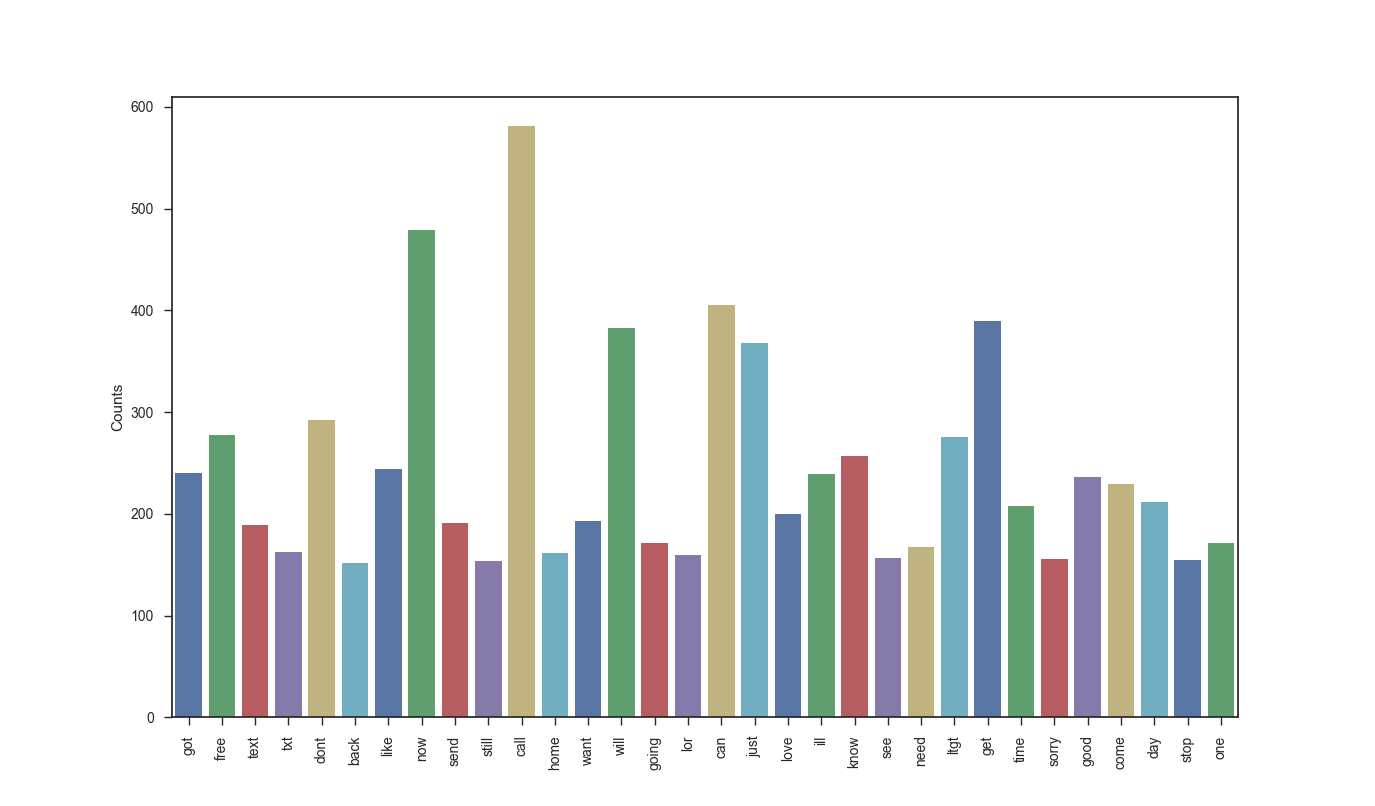
\includegraphics[width=\textwidth]{word_barplot.png}
    \caption[Figura simples]{Gráfico de barras com frequências de palavras mais comuns de 
    \texttt{SMS} superiores a 150.}
    \label{fig:barplot}
\end{figure}

O gráfico mostra 32 palavras com ocorrência superior ao mínimo estabelecido (para efeito de melhor
visualização). A lista completa destas palavras é: \texttt{got, free, text, txt, dont, back, 
like, now, send, still, call, home, want, will, going, lor, can, just, love, ill, know, see, need, 
ltgt, get, time, sorry, good, come, day, stop, one}.

Um outro recurso de mais fácil visualização é a nuvem de palavras. Nela, o tamanho de cada palavra 
é proporcional a sua frequência de ocorrência. Neste caso uma nuvem de palavras foi aplicada sobre 
o universo de palavras mais comuns. A figura \ref{fig:wordcloud} apresenta a nuvem com as 50 palavras 
de maior ocorrência. Através do recurso de nuvem fica muito mais fácil identificar, por exemplo,
que as palavras mais utilizadas foram: \texttt{call, can, now, will, get, just}.


\begin{figure}[htbp]
    \centering
    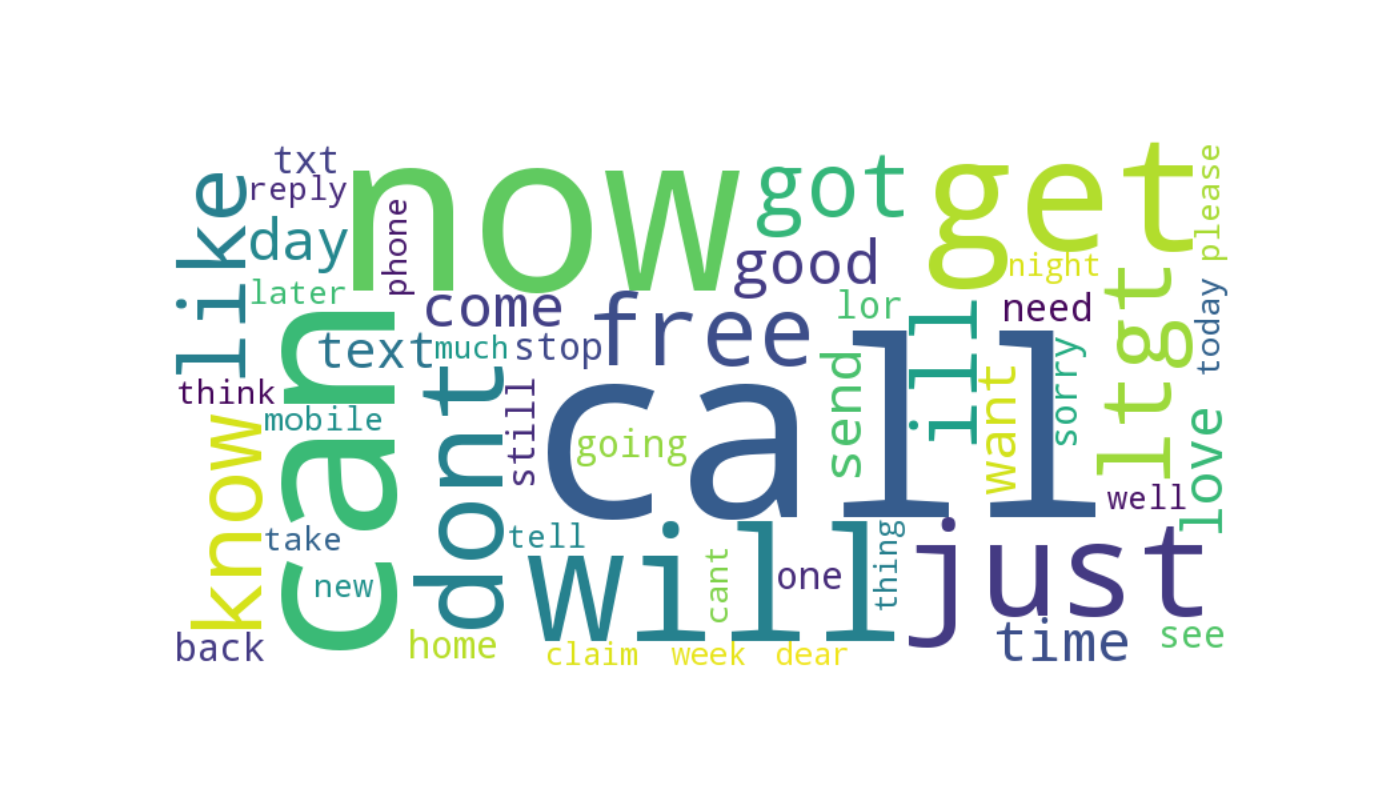
\includegraphics[width=\textwidth]{word_cloud.png}
    \caption[Figura simples]{Nuvem com as 50 palavras mais frequentes dentro de um universo de 
    palvras mais comuns de \texttt{SMS}.}
    \label{fig:wordcloud}
\end{figure}


\newpage
A seguir, foi feita uma análise da quantidade de mensagens normais e de spam por mês. O 
gráfico de barras na figura \ref{fig:monthly_spam} apresenta estas quantidades para os meses de Janeiro, Fevereiro 
e Março. É possível ver que o número de mensagens classificadas como ``spam'' é bem reduzido 
quando comparado ao número de mensagens comuns. O número de spams aparenta posuir mais 
homogeneidade e uma frequência superior a 200 vezes por mês.


\begin{figure}[htbp]
    \centering
    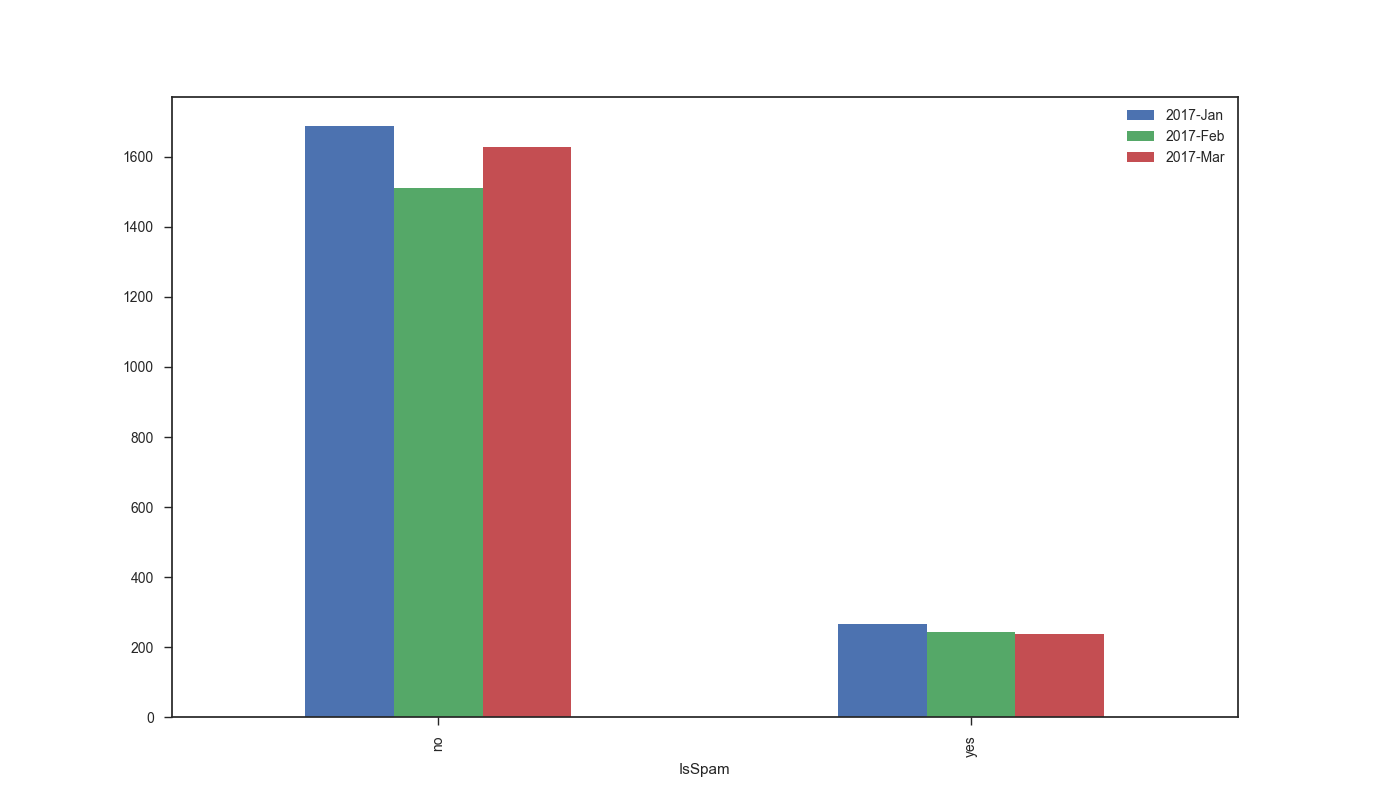
\includegraphics[width=\textwidth]{monthly_spam.png}
    \caption[Figura simples]{Número mensal de mensagens comuns vs. spams para \texttt{SMS}.}
    \label{fig:monthly_spam}
\end{figure}


Para o atributo \texttt{Word\_Count}, um número de estatísticas descritivas foram calculadas: 
max, min, média, mediana e desvio padrão. A tabela \ref{tab:stats} apresenta o cenário encontrado para
esta variável.



\vspace{.5cm}
% \newpage
\makesavenoteenv{tabular}
\begin{center}
\captionof{table}{Diferentes estatísticas encontradas para o atributo \texttt{Word\_Count}.}
\begin{tabular}{cccccc}
 \hline
            &  \textbf{min.} &  \textbf{max.}  &  \textbf{média}  & \textbf{mediana}  & \textbf{desvio padrão}\\
  2017-Jan  &  2    &  190  &  16.34  &  13  &  12.56 \\
  2017-Fev  &  2    &  100  &  16.03  &  13  &  11.04  \\
  2017-Mar  &  2    &  115  &  16.28  &  12  &  11.58  \\
 \hline
%  \hline
 \label{tab:stats}
\end{tabular}
\end{center}

Observa-se uma característica de dispersão de valores em torno de medidas de centralidade, uma vez 
que o desvio padrão é comparável aos valores de média/mediana. O fato da média ser um pouco maior 
que a mediana indica a existência de algumas mensagens muito longas (com muitas palavras). Isto
está de acordo pois o valor máximo encontrado para esta variável é sempre superior a 100 palavras,
o que acaba deslocando o valor da média nesta direção.



\newpage

\vspace{1cm}

\subsection{Validação cruzada usando ``k-pastas''}
A tabela \ref{tab:metrics} apresenta os valores médios e erro associado das métricas de avaliação 
de desempenho f1-score, \textit{precision} (precisão) e \textit{recall} (revocação) encontrados 
aplicando validação cruzada com 10 pastas. A tabela \ref{tab:tempo} indica os tempos registrados 
em cada etapa realizado de forma independente. É possível ver que os melhores desempenhos gerais 
ocorrem para modelos mais complexos (SVM e MLP) com valores do f1-score comparáveis dentro da 
margem de erro. A complexidade de cada modelo está normalmente associado ao custo computacional 
que reflete no tempo de cada processo. No entanto, não necessariamente o modelo mais complexo irá 
apresentar desempenho superior. Isto é visível para o tempo de resposta do modelo de SVM 
da validação cruzada é muito menor (próximo a 16 segundos) quando comparado ao modelo MLP 
(acima de 1 minuto).


\vspace{.5cm}
% \newpage
% \makesavenoteenv{tabular}
\begin{center}
\captionof{table}{Estimativas de métricas de desempenho para os modelos de classificação usados.}
\begin{tabular}{cccc}
 \hline
	        &  \textbf{f1-score}  & \textbf{precisão}  & \textbf{revocação} \\
 Naïve-Bayes	&  0,840 ($\pm$ 0,072) & \textbf{1,00} ($\pm$ 0,000)  & 0.726 ($\pm$ 0,104) \\
 Regressão logística & 0,805 ($\pm$ 0,069) & 0,989 ($\pm$ 0,031) & 0,680 ($\pm$ 0,095) \\
 SVM            &  0,942 ($\pm$ 0,048) & 0,987 ($\pm$ 0,032) & 0,901 ($\pm$ 0,070)  \\
 MLP 		&  \textbf{0,943} ($\pm$ 0,027) & 0,963 ($\pm$ 0,046) & \textbf{0,924} ($\pm$ 0,052)  \\
 \hline
%  \hline
 \label{tab:metrics}
\end{tabular}
\end{center}





\vspace{.5cm}
% \newpage
% \makesavenoteenv{tabular}
\begin{center}
\captionof{table}{Tempos registrados para o processo de validação cruzada com 10 pastas.}
\begin{tabular}{cccc}
 \hline
	        &  \textbf{f1-score}  & \textbf{precisão}  & \textbf{revocação} \\
 Naïve-Bayes	&  8,912 s 	 & 8,971 s  	& 8,949 s \\
 Regressão logística & 9,228 s 	 & 9,076 s  	& 9,073 s  \\
 SVM            &  16,295 s 	 & 16,283 s 	& 16,293 s \\
 MLP 		&  \textbf{73,721 s}  & \textbf{74,789 s}   & \textbf{72,395 s}  \\
 \hline
%  \hline
 \label{tab:tempo}
\end{tabular}
\end{center}




\section{Conclusão}




 
\end{document}


